% !TEX encoding = UTF-8 Unicode
\newcommand{\aktion}[1]{ \subsubsection{#1} }
\newcommand{\bParameterlist}{\begin{tabular}[t]{l|p{3.3cm}|l} parameter & range & function \\ \hline }
\newcommand{\param}[4]{\emph{#1} & \emph{#2} ... \emph{#3} & \emph{#4} \\}
\newcommand{\paramSw}[4]{\emph{#1} & \emph{#2} / \emph{#3} & \emph{#4} \\}
\newcommand{\paramRe}[6]{\emph{#1} & \emph{#2}...\emph{#3} or \emph{#4}...\emph{#5} & \emph{#6} \\}
\newcommand{\eParameterlist}{\end{tabular}\\\\}


\kap{Modules}
VSTForx knows three types of modules: 
\begin{itemize}
	\item signal processor
	\item signal switch
	\item signal transformer
\end{itemize}
%%%%%%%%%%%%%%%%%%%%%%%%%%%%%%%%%%%%%%%%%%%%%%%%%%%%%%%%%%%%%%%%%%%%%%%%%%%%%%%%
\ukap{Common Module Parameters}
\aktion{MIDI}
Every modules/plugins which are able to receive midi data have an additional \emph{'midi-channel'} parameter:\\
\bParameterlist
	\param{midi\_channel}{all, 0}{16}{selects the receiving midi channel }
\eParameterlist


%%%%%%%%%%%%%%%%%%%%%%%%%%%%%%%%%%%%%%%%%%%%%%%%%%%%%%%%%%%%%%%%%%%%%%%%%%%%%%%%
\ukap{Volume}
The Volume module is a signal processor. It contains a single parameter which allows to control the volume of the incoming signal.
\aktion{Module Parameter}
	\bParameterlist
		\param{Volume}{0}{1}{controls the volume}
	\eParameterlist

%%%%%%%%%%%%%%%%%%%%%%%%%%%%%%%%%%%%%%%%%%%%%%%%%%%%%%%%%%%%%%%%%%%%%%%%%%%%%%%%
\ukap{Pan}
Like the Volume module, the Pan module is a signal processor with a single parameter. Use it to control the panning of the incoming signal.
\aktion{Modul Parameter}
	\bParameterlist
		\param{Pan}{0}{1}{controls the pan}
	\eParameterlist
%%%%%%%%%%%%%%%%%%%%%%%%%%%%%%%%%%%%%%%%%%%%%%%%%%%%%%%%%%%%%%%%%%%%%%%%%%%%%%%%
\ukap{Input / Output Switches} 
Input / Output Switches are able to switch between several states while every state belongs to an input respectively to an output. An "Input Switch" for example can switch several inputs to one output. A "selector" parameter controls the switch state. Furthermore several parameters control the "fade-in / fade-out" behaveiour.
\aktion{Adding States}
	To add an additional switch state you can find a respective option in the context menu of any switch object.  
\aktion{Module Parameters}
	\bParameterlist
		\param{selector switch}{0}{1}{the state selector}
		\param{fade-in duration x\stern}{0ms}{1000ms}{''fadein'' duration x}
		\param{fade-in curve type x\stern}{type1}{type\sstern}{''fadein'' slope type x}
		\param{fade-out duration x\stern}{0ms}{1000ms}{''fadeout'' duration x}
		\param{fade-out curve type x\stern}{type1}{type\sstern}{''fadeout'' slope type x}
	\eParameterlist
\stern : x=the related state \\
\sstern : see figure \ref{curvetypes} on page \pageref{curvetypes}

%%%%%%%%%%%%%%%%%%%%%%%%%%%%%%%%%%%%%%%%%%%%%%%%%%%%%%%%%%%%%%%%%%%%%%%%%%%%%%%%
\ukap{Input/Output Step Switches} 
Unlike the "I/O Switches" the "Step Switch" state is not controlled by a parameter. The states will be iterated automatically. Either with a \emph{fixed} time per state or \emph{synced} to the beat of the current DAW.\\
\\\\
\tip{%Wann der Syncmodus die Stepsequenz beginnt, ist abhängig davon, an welcher Taktposition in der Hostanwendung die Start-Taste gedrückt wurde. Gestartet wird immer an dem nächst liegenden Viertelnotenwert.
Heads Up! In sync mode the state position will be reseted on incoming "play" event of the DAW. }
\aktion{Adding States}
	To add an additional switch state you can find a respective option in the context menu of any switch object.   
\aktion{Module Parameters}
	\bParameterlist
		\paramSw{Step Type}{fix}{sync}{Der Step Modus}
		\paramRe{Step x duration\stern}{10ms}{1000ms}{1/128}{1/1\sstern}{duration x}
		\param{fade-in duration x\stern}{0ms}{1000ms}{''fadein'' duration x}
		\param{fade-in curve type x\stern}{type1}{type\ssstern}{''fadein'' slope type x}
		\param{fade-out duration x\stern}{0ms}{1000ms}{''fadeout'' duration x}
		\param{fade-out curve type x\stern}{type1}{type\ssstern}{''fadeout'' slope type x}
	\eParameterlist
\stern : x=the related state \\
\sstern : see figure \ref{curvetypes} on page \pageref{curvetypes}
%%%%%%%%%%%%%%%%%%%%%%%%%%%%%%%%%%%%%%%%%%%%%%%%%%%%%%%%%%%%%%%%%%%%%%%%%%%%%%%%
\ukap{Peak Transformer}
The peak transformer transforms incoming audio peaks into an output parameter value.
\aktion{Module Parameters}
	\bParameterlist
		\param{out}{0}{1}{the output value}
		\param{offset}{0}{1}{offset to the output value}
	\eParameterlist
%%%%%%%%%%%%%%%%%%%%%%%%%%%%%%%%%%%%%%%%%%%%%%%%%%%%%%%%%%%%%%%%%%%%%%%%%%%%%%%%
\ukap{ADSR Trigger}
The ADSR Trigger generates an ADSR (figure \ref{adsr} on page \pageref{adsr}) sequence triggered by an audio signal. This sequence will be transformed into an output parameter value. Thus it's possible to control parameters (or rather the connected units) with any audio input.
\aktion{Module Parameters}
	\bParameterlist
		\param{out}{0}{1}{the output value}
		\param{x level\stern}{0}{1}{final value of x}
		\param{x duration\stern}{0s}{5s}{duration of x}
		\param{x slope type\stern}{type1}{type6\sstern}{slope type x}
		\param{trigger\_threshold}{0}{1}{trigger threshold}
		\param{trigger\_hold}{0}{5s}{determines the minimum retain duration of the trigger}
	\eParameterlist
\stern : x=the related state: attack, decay, sustain, release \\
\sstern : see figure \ref{curvetypes} on page \pageref{curvetypes}
%%%%%%%%%%%%%%%%%%%%%%%%%%%%%%%%%%%%%%%%%%%%%%%%%%%%%%%%%%%%%%%%%%%%%%%%%%%%%%%%
\ukap{MIDI Receiver}
The MIDI Receiver is a transformer module. It transforms MIDI signals into parameter values.
\aktion{Module Parameters}
127 MIDI control + pitchbend parameter. 

\ukap{Appendix}

\begin{figure}[pth]
\begin{center}
	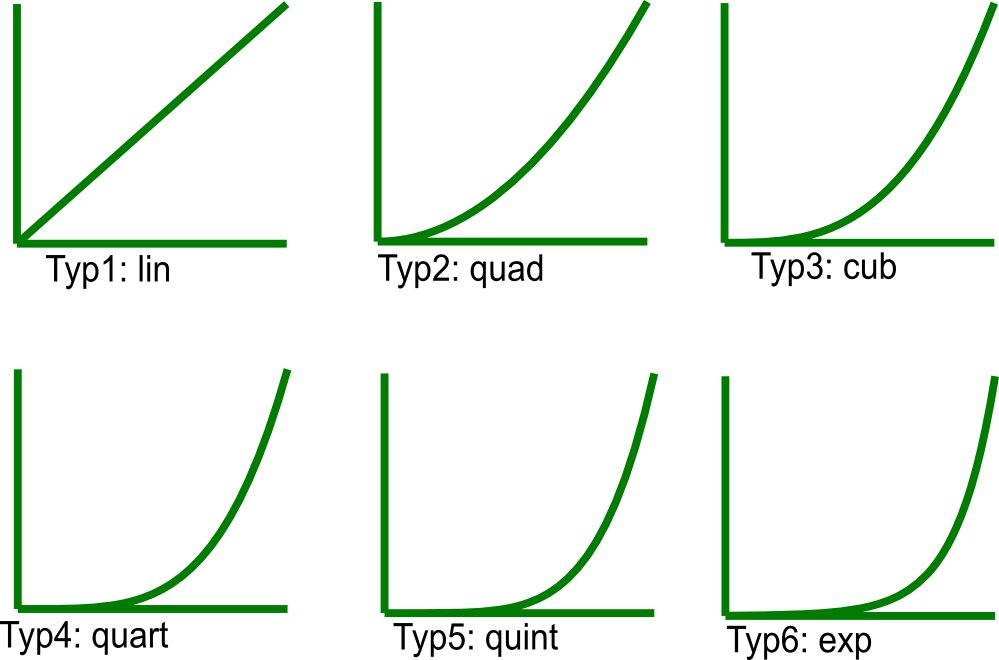
\includegraphics[scale=1.4]{../graphics/curvetypes}
\caption{the six slope types of VSTForx}
\label{curvetypes}
\end{center}
\end{figure}

\begin{figure}[pth]
\begin{center}
	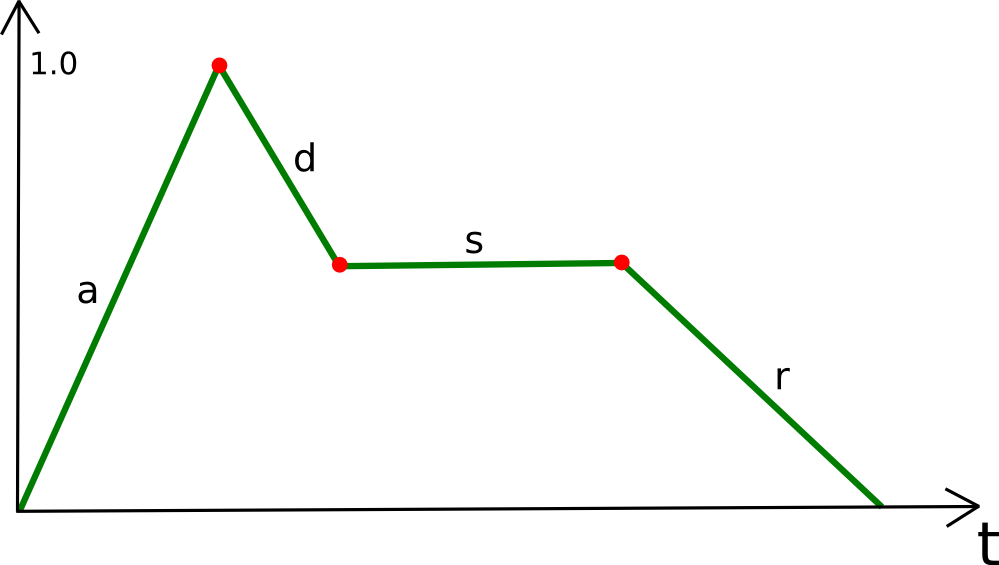
\includegraphics[scale=1.4]{../graphics/adsr}
\caption{example of an ADSR curve}
\label{adsr}
\end{center}
\end{figure}
